\chapter{Unmodified band structure\label{chap:TB}}
Graphene's linear electronic dispersion was first investigated by Wallace \cite{Wallace1947}, fifty seven years before Geim, Novoselov and co-workers spurred graphene research forward with their method of mechanical exfoliation \cite{Novoselov2004}.
Thirty seven years later Semenoff formalized the equivalence between the low energy electrons in graphene and relativistic Dirac-Weyl electrons \cite{Semenoff1984}.
Remarkably, the fairly simple nearest neighbor tight binding approach used by these authors has accurately described the majority of the low energy physics in graphene.
This chapter will follow in the spirit of these derivations but include additional emphasis to guide the discussions of the strain induced pseudovector potentials and the phonon induced Kekul\'e transition.

\section{Graphene's lattice and Brillouin zone \label{sec:TB:geom}}
\begin{figure}
	\begin{center}
	{
% Geometry taken directly from my lectures notes on tight binding in graphene
\newcommand{\alat}{1 cm}
\newcommand{\sqth}{1.73205080757}
\newcommand{\Klen}{2 cm}
\begin{tikzpicture}															

	% Graphene lattice, sublattices different colors, nearest neighbor vectors and lattice vectors
	\begin{scope}[xshift=-3.75 cm,>=stealth,
		nnarrow/.style={color=black,very thick, ->},					% Nearest neighbor vectors
		B/.style={circle,draw=blue!50,fill=blue!20,
			thick,minimum size=2 mm,inner sep=0pt}, 					% A sublattice dots
		A/.style={circle,draw=orange!70,fill=orange!40,
			thick,minimum size=2mm,inner sep=0pt},						% B sublattice dots
		el1/.style={x radius=.3*\alat,y radius=.85*\alat},				% Style for the ellipse
		el2/.style={dashed,thick,draw=black!75}]						% Style for the ellipse draw

		%This scope is clipped to limit the drawn lattice to a square
		\clip (-3.9cm,-4.38cm) rectangle(3.9cm,3cm);
		% Draw the lattice
		\foreach \ip in {-3,-2,...,3}
			\foreach \im in {-3,-2,...,3}
			{
			\node at (\ip*\sqth*\alat/2-\im*\sqth*\alat/2, \ip*\alat*3/2+\im*\alat*3/2+\alat/2) [A] {};
			\node at (\ip*\sqth*\alat/2-\im*\sqth*\alat/2, \ip*\alat*3/2+\im*\alat*3/2-\alat/2) [B] {};
			}

		% Draw the nearest neighbor vectors
		\draw[nnarrow] (60:\alat*\sqth)++(-30:\alat)++(0,-\alat/2) -- +(270:\alat) node[anchor=north     ]{$\vec{\delta}_1$};
		\draw[nnarrow] (60:\alat*\sqth)++(-30:\alat)++(0,-\alat/2) -- +( 30:\alat) node[anchor=south west]{$\vec{\delta}_2$};
		\draw[nnarrow] (60:\alat*\sqth)++(-30:\alat)++(0,-\alat/2) -- +(150:\alat) node[anchor=south east]{$\vec{\delta}_3$};
		
		% Draw the lattice vectors
		\draw[nnarrow] (240:2*\sqth*\alat) --node[circle,anchor=north west]{$\vec{a}_+$} +( 60:\sqth*\alat) ;
		\draw[nnarrow] (240:2*\sqth*\alat) --node[circle,anchor=north east]{$\vec{a}_-$} +(120:\sqth*\alat);

		% Ellipses around two atom basis
		\draw[el2] (240:2*\sqth*\alat) +(  0,0          ) ellipse[el1];
		\draw[el2] (240:2*\sqth*\alat) +( 60:\sqth*\alat) ellipse[el1];
		\draw[el2] (240:2*\sqth*\alat) +(120:\sqth*\alat) ellipse[el1];
	\end{scope}

	% Reciprocal space BZ and high symmetry points
	\begin{scope}[xshift=3.75cm,yshift=-1 cm,
		BZ/.style={color=black,fill=black,very thick},
		Bar/.style={color=black,very thick,->},
		circ2/.style={radius=1.5pt}]

		% Draw the BZ
		\draw[BZ]
			(  0:\Klen) circle[circ2] node[anchor=west      ]{$\bm{K} $} --
			( 60:\Klen) circle[circ2] node[anchor=south west]{$\bm{K'}$} --
			(120:\Klen) circle[circ2] node[anchor=south east]{$\bm{K }$} -- 
			(180:\Klen) circle[circ2] node[anchor=east      ]{$\bm{K'}$} -- 
			(240:\Klen) circle[circ2] node[anchor=north east]{$\bm{K }$} -- 
			(300:\Klen) circle[circ2] node[anchor=north west]{$\bm{K'}$} -- 
			(  0:\Klen);

		% Label the high symmetry points
		\draw[BZ] (0,0) circle[circ2] node[anchor=west]{$\Gamma$};

		% The primitive RLVs
		\draw[Bar] (0,0) -- ( 30:\sqth*\Klen) node[anchor=south east]{$\vec{b}_+$};
		\draw[Bar] (0,0) -- (150:\sqth*\Klen) node[anchor=south west]{$\vec{b}_-$};
	\end{scope}

	% (a) and (b) labels
	\node at (-7cm,3.5cm) {\textbf{(a)}};
	\node at ( 1cm,3.5cm) {\textbf{(b)}};
\end{tikzpicture}
}
	\end{center}
	\caption[Geometry of intrinsic graphene]{\label{fig:TB:geometry} Geometry of intrinsic graphene.  (a) Real space graphene lattice with the A sub-lattice in orange, the B sub-lattice in blue, nearest neighbor vectors ($\vec \delta_1$, $\vec \delta_2$, and $\vec \delta_3$) shown as arrows, and lattice vectors ($\vec a_+$ and $\vec a_-$) shown translating the two atom basis. (b) First Brillouin zone with labeled high symmetry points and reciprocal lattice vectors ($\vec{b}_+$ and $\vec{b}_-$).}
\end{figure}

In its unperturbed state the carbon atoms in the graphene lattice are arrayed in a hexagon as shown in Figure \ref{fig:TB:geometry}(a).
Throughout this thesis the $\hat x$ direction will be oriented along the zigzag direction as shown.
Since a hexagonal lattice is not a Bravais lattice, the lattice must be treated as a triangular Bravais lattice with a two atom bases.
In Figure \ref{fig:TB:geometry}(a) the A sub-lattice is colored orange and the B sub-lattice is colored blue.
The lattice is created by arraying the two atoms basis using the primitive lattice vectors 
\begin{align*}
	\vec{a}_+&= \frac{\sqrt{3}a}{2} \left( +\hat{x} + \sqrt{3} \ \hat{y} \right) \\
	\vec{a}_-&= \frac{\sqrt{3}a}{2} \left( -\hat{x} + \sqrt{3} \ \hat{y} \right) \ ,
\end{align*}
where $a=1.4 \ \angstrom$ is the nearest neighbor distance.
The three nearest neighbor vectors,
\begin{align*}
	\vec \delta_1&=-a \hat{y} \\
	\vec \delta_2&= \frac{a}{2} \left( +\sqrt{3} \ \hat{x}+\hat{y} \right)\\
	\vec \delta_3&= \frac{a}{2} \left( -\sqrt{3} \ \hat{x}+\hat{y} \right) \ ,
\end{align*}
connect each atom in the A sub-lattice to its three nearest neighbors in the B sub-lattice.

Graphene's reciprocal lattice is shown in Figure \ref{fig:TB:geometry}(b).
The primitive reciprocal lattice vectors, 
\begin{align*}
	b_+&=\frac{2 \pi}{3} \left(+\sqrt{3} \ \hat{x} + \hat{y} \right) \\ 
	b_-&=\frac{2 \pi}{3} \left(-\sqrt{3} \ \hat{x} + \hat{y} \right) \ ,
\end{align*} 
create the hexagonal first Brillouin zone (BZ).
The hexagon is rotated 30 degrees relative to the real space hexagonal lattice.
The $\Gamma$ point is at the center of the Brillouin zone while the $\bm{K}$ and $\bm{K'}$ are at the corners.
Only 2 of the 6 corners of the hexagon are unique, the others can be connected by reciprocal lattice vectors.
The two unique corners are referred to as $\bm{K}$ and $\bm{K'}$ are positioned at
\begin{align*}
	\bm{K}&=-\bm{K'}= \frac{4 \pi}{3 \sqrt{3} a} \hat{x} \\
	\bm{K}&=-\bm{K'}= \frac{2 \pi}{3 \sqrt{3} a} \left( -1 \ \hat{x} + \sqrt{3} \hat{y} \right)\\
	\bm{K}&=-\bm{K'}= \frac{2 \pi}{3 \sqrt{3} a} \left( -1 \ \hat{x} - \sqrt{3} \hat{y} \right) \ .
\end{align*}
For simplicity we will often work with the first pair.

In later sections this discussion will be expanded to take into account strain and phonons which modify the graphene lattice.
In both cases the changes in graphene's electronic dispersion are directly linked to geometric distortions.

\section{Tight binding motivation}
The tight binding formalism is used universally in this work.
As such, it will be briefly motivated here.
Afterward, the nearest neighbor tight binding formalism will be applied to graphene.

In second quantization the total electronic energy in the system is written as
\begin{equation*}
	H=\sum_{\vec{k}} c^{\dagger}_{\vec{k}} c_{\vec{k}} \epsilon_{\vec{k}} \ ,
\end{equation*}
where $c^{\dagger}_{\vec{k}}$ and $c_{\vec{k}}$ are the creation and annihilation operators for an electron with wavevector $\vec{k}$ and energy $\epsilon_{\vec{k}}$.
The product $c^{\dagger}_{\vec{k}} c_{\vec{k}}$ is the number operator which counts the number of electrons with the given wavevector.
Thus, the energy is found by simply summing the energy of each electron.

When the atomic wave functions of the atoms in the material do not overlap considerably it is reasonable to work with real space creation and annihilation operators.
These operators create or annihilate electrons at specific lattice points.
The reciprocal space operators are related to the real space operators through a Fourier transform
\begin{align*}
	c^{\dagger}_{\vec{k}}&=\frac{1}{\sqrt{N}}\sum_{\vec{R}_i} e^{ i \vec{k} \cdot \vec{R}_i} c^{\dagger}_{i} \\
	c          _{\vec{k}}&=\frac{1}{\sqrt{N}}\sum_{\vec{R}_j} e^{-i \vec{k} \cdot \vec{R}_j} c_{j} \ ,
\end{align*}
where the sum is over the lattice vectors.
This Fourier transform can only eliminate spatial dependencies with the periodicity of the lattice.
As such, if there are more than one atom per unit cell distinct creation and annihilation operators must be used for each atom in the basis.

Applying the Fourier transform to the systems Hamiltonian yields the tight binding Hamiltonian
\begin{align*}
	H&=-\sum_{\vec{R}_i, \vec{R}_j} (-) \sum_{\vec{k}}\frac{1}{N} e^{i \vec{k} \cdot (\vec{R}_i-\vec{R}_j)}
	 \epsilon_{\vec{k}} c^{\dagger}_{i} c_{j} \\
	 &\approx -\sum_{<i,j>} t_{i,j} c^{\dagger}_{i} c_{j} + \text{H.C} \ .
\end{align*}
By limiting the sums to the $<i,j>$ nearest neighbor pairs we are limiting ourselves to a nearest neighbor tight binding formalism.
The hopping energy, $t_{i,j}=-\sum_{\vec{k}}\frac{1}{N} e^{i \vec{k} \cdot (\vec{R}_i-\vec{R}_j)}\epsilon_{\vec{k}}$, is the energy associated with removing an electron from atom $j$ and putting it on atom $i$.
It is usually determined empirically or calculated by matching the tight binding model to other more powerful methods such as density functional theory.
In graphene, it is around 2.8 eV \cite{CastroNeto2009}.

By using real space creation and annihilation operators the reciprocal space Hamiltonian has been recast into real space.
As will be shown for graphene, this proves to be a powerful starting point.

\section{Tight binding in graphene \label{sec:TB:TB}}
\subsection{Nearest neighbor tight binding}
The physics relevant for this work is captured by the nearest neighbor tight binding formalism.
In graphene, when an electron hops between nearest neighbor it changes sub-lattice.
This is reflected in the nearest neighbor tight binding Hamiltonian,
\begin{equation}
	H=-t_0 \sum_{<i,j>} (a_i^{\dagger} b_j + \text{H.C.}) \ .
	\label{eq:TB:baseham}
\end{equation}
Here the hopping energy, $t_0$, gives the energy required to remove an electron from the $j$th atom in the B sub-lattice using the B sub-lattice annihilation operator, $b_j$, and put that electron on it nearest neighbor, the $i$th atom in the A sub-lattice using the A sub-lattice creation operator, $a_i$.
The hopping from the A sub-lattice back to the B sub-lattice is taken into account by the the Hermitian conjugate, $\text{H.C.}$.

The Hamiltonian is simplified by writing the creation and annihilation operators in Fourier space using a Fourier expansion.
There is some freedom in choosing the phase factors in the Fourier expansion.
The operators can be expanded around the atomic positions or, alternatively, they can be expanded around the position of the basis occupied by the atom.
Both approaches yield the same result if one is consistent \cite{Bena2009}.
Throughout this thesis we will expand about the atomic basis.
This will make the correspondence with the Dirac-Weyl equation more clear.
The expanded operators are
\begin{align}
	a_i^{\dagger}&=\frac{1}{\sqrt{N}}\sum_{\vec{k} } e^{ i \vec{k}  \cdot \vec{R}_i} a_{\vec{k} }^{\dagger} \nonumber \\
	b_j          &=\frac{1}{\sqrt{N}}\sum_{\vec{k}'} e^{-i \vec{k}' \cdot \vec{R}_j} b_{\vec{k}'} \ ,
	\label{eq:TB:FT} 
\end{align}
where $R_i$ and $R_j$ are the position of the $i$th and $j$th atomic basis respectfully.  
The nearest neighbor is either in the same atomic basis or in one of the neighboring atomic bases.
Thus, $\vec{R}_j$ is restricted to $\vec{R}_j \in \{ \vec{R}_i,\vec{R}_i+\vec{a}_+,\vec{R}_i+\vec{a}_-\}$ and the difference $\vec{\Delta_j}=\vec{R}_j-\vec{R}_i$ is independent of $i$.
In reciprocal space the Hamiltonian becomes
\begin{align}
	H&=-t_0 \frac{1}{N} \sum_{\vec{k},\vec{k'}}\sum_i\sum_j \left( e^{i (\vec{k}-\vec{k}') \cdot \vec{R}_i}
		e^{-i \vec{k}' \cdot \vec{\Delta}_j}
		a^{\dagger}_{\vec{k}} b_{\vec{k}'} + \text{H.C.} \right) \nonumber \\
	 &=-t_0 \frac{1}{N} \sum_{\vec{k},\vec{k'}}\sum_j \left( N \delta_{\vec{k},\vec{k'}} \
	 	e^{-i \vec{k}' \cdot \vec{\Delta}_j}
		a^{\dagger}_{\vec{k}} b_{\vec{k}'} + \text{H.C.}\right) \nonumber \\ 
	 &=-t_0 \sum_{\vec{k}}\left( \sum_{j} e^{-i \vec{k} \cdot \vec{\Delta}_j} a^{\dagger}_{\vec{k}} b_{\vec{k}} + \text{H.C.} \right) \label{eq:TB:FTing}\ ,
\end{align}
where $\delta_{\vec{k},\vec{k'}}$ is the Kronecker delta function.
In matrix notation this reads
\begin{equation}
	H=\sum_{\vec k} 
		\left( \begin{array}{cc} a^{\dagger}_{\vec{k}} & b^{\dagger}_{\vec{k}} \end{array} \right)
		\left( \begin{array}{cc}
			0              & -t_0 \sum_{j} e^{-i \vec{k} \cdot \vec{\Delta}_j} \\
			-t_0 \sum_{j} e^{-i \vec{k} \cdot \vec{\Delta}_j} & 0               \end{array} \right)
		\left( \begin{array}{c } a_{\vec{k}}           \\ b_{\vec{k}}          \end{array} \right) \ .
	\label{eq:TB:fullH}
\end{equation}
The two atom basis yields a two by two matrix which will give two energy bands.

A straightforward calculation provides the electron dispersion,
\begin{equation*}
	E(\vec{k})=\pm t_0 |h(\vec{k})|=t_0 \sqrt{1+4 \cos^2 \left(\frac{\sqrt{3}}{2} a k_x\right)
		+4 \cos\left(\frac{\sqrt{3}}{2} a k_x \right) \cos \left(\frac{3}{2} a k_y\right)} \ ,
\end{equation*}
which is plotted in Figure \ref{fig:TB:Dispersion}.
As shown, the two energy bands touch at the corners of the Brillouin zone.
For pristine graphene there is one electron per carbon atom leaving the low energy band completely filled and the high energy band empty.
The points where the bands meet are referred to as the Dirac points or as the charge neutrality points.
The Fermi energy can be shifted by charge transfer from contaminates or it can be purposely modified by adding or removing charges through capacitive coupling.
The resulting shifts in Fermi energy are relatively small and, thus, the low energy excitations happen in a narrow energy window around these points.
This happens to be the energy window for which the nearest neighbor tight binding approach is most accurate.
A higher order model is required to account for things such as trigonal warping which alter the dispersion at higher energies.

\begin{figure}
	\begin{center}
	\begin{tikzpicture}
	\node at (0,0) {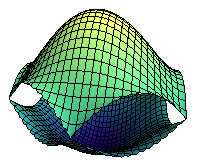
\includegraphics{Figs_TightBinding/bandstructure_3.png}};
	\node at (-3.75,-.5) {$\bm{K}$};
	\node at (-.25,-2)[fill=white, rounded corners]{$\bm{K'}$};
\end{tikzpicture}
	\end{center}
	\caption[Electronic dispersion of intrinsic graphene]{\label{fig:TB:Dispersion} The electronic dispersion of intrinsic graphene in the BZ calculated with a nearest neighbor tight binding model.  The two energy bands meet at the $\bm{K}$ and $\bm{K'}$ points.}	
\end{figure}

\subsection{Low energy approximation}
The two points of convergence between the high and low energy bands are referred to as the Dirac points because of the characteristic energy dispersion in their vicinity.
This interesting low energy physics is best captured by expanding the Hamiltonian in Equation \ref{eq:TB:fullH} about these points.
The wavevectors are approximated as $\vec{k}=\bm{K}+\vec{q}$ and $\vec{k}=\bm{K'}+\vec{q}$.
For small $qa$ the sum in Equation \ref{eq:TB:fullH} is approximately
\begin{align}
	\sum_{j} e^{-i \vec{k} \cdot \vec{\Delta}_j}&= \nonumber \\
	\bm{K:}\ 	&\simeq \sum_{j} (1-i \vec{q} \cdot \vec{\Delta}_j) e^{-i \bm{K} \cdot \vec{\Delta}_j} \nonumber \\
				&=-\frac{3}{2} a \left( q_x-i q_y \right) \nonumber \\
	\bm{K':}\	&\simeq \sum_{j} (1-i \vec{q} \cdot \vec{\Delta}_j) e^{-i \bm{K'} \cdot \vec{\Delta}_j} \nonumber \\
				&=-\frac{3}{2} a \left(-q_x-i q_y \right) \ .
	\label{eq:TB:LowEnergy} 
\end{align}
These expansions are independent of which of the three identical $\bm{K}$ or $\bm{K'}$ points are selected.
The approximate low energy Hamiltonians near the $\bm{K}$ and $\bm{K'}$ points can be combined into a single Hamiltonian
\begin{align}
	H&=\hbar v_f \sum_{\vec q, \vec{q}}
		\psi^{\dagger}
		\left( \begin{array}{cccc}
			0              & q_x - i q_y & 0            & 0 \\
			q_x+i q_y      & 0           & 0            & 0 \\                            
			0              & 0           & 0            & -q_x+i q_y \\
			0              & 0           & -q_x-i q_y & 0			            			\end{array} \right)
		\psi \nonumber \\
	H&=\sum_{\vec q, \vec{q}}
		\psi^{\dagger}
		\left( \begin{array}{cc}
			v_f \vec{p} \cdot \vec{\sigma}              & 0\\
			0              & -v_f \vec{p} \cdot \vec{\sigma}			   	            			\end{array} \right)
		\psi \ ,
	\label{eq:TB:FullH}
\end{align}
where 
\begin{equation}
\psi^{\dagger}=(a^{\dagger}_{\vec{q}}, b^{\dagger}_{\vec{q}},  b^{\dagger}_{\vec{q}}, a^{\dagger}_{\vec{q}})
\label{eq:TB:spinor}
\end{equation}
is the combined wave function, $\vec{\sigma}= \left( \begin{array}{cc} 0 & 1 \\ 1 & 0 \end{array} \right) \hat{x}+\left( \begin{array}{cc} 0 & -i \\ i & 0 \end{array} \right) \hat{y}$ is the vector of Pauli matrices, and $v_f$ is the Fermi velocity given by $\frac{3}{2}\frac{at}{\hbar} \sim .9 \times 10^6 \ m/s$.
In order to express the Hamiltonian near the $\bm{K'}$ point in terms of Pauli matrices, the order of the second pair of raising and lowering operators in $\psi$ had to be switched.
The approximate low energy Hamiltonian will be central for the discussion of electron physics in manipulated graphene.

At both $\bm{K}$ and $\bm{K'}$ the low energy electronic dispersion is identical
\begin{equation*}
	E=\pm \hbar v_f |\vec{q}| \ .
\end{equation*}
This linear canonical energy dispersion is reminiscent of the linear dispersion exhibited by photons.

The density of electronic states can be calculated from the low energy dispersion.
Taking account the two fold spin and two fold valley degeneracy, the density of states is 
\begin{equation}
	\rho(\epsilon)=\frac{2}{\pi} \left( \frac{\hbar v_f}{L} \right)^2 \epsilon \ ,
	\label{eq:TB:DOS}
\end{equation}
where $L^2$ is the area of the graphene and $\epsilon$ is the energy measured from the charge neutrality point.
The density of states at a given energy goes as the circumference of the Dirac cone resulting in a linear energy dependence.

\section{Dirac-Weyl electrons}
Graphene's linear electrical dispersion is peculiar.
According to the usual, non-relativistic expression for the effective mass of an electron in an electric field, $m^*=\frac{\hbar^2}{\left(\frac{d^2 E}{d k^2}\right)}$ \cite{Kittel2005}, the electrons in graphene have an infinite effective mass.
In a classical sense, this interpretation makes sense.
The electron's group velocity, $d \omega/d k$, is independent of momentum, and thus, as if it had an infinite mass, an electron's velocity cannot be changed by applying a force.
However, a relativistic interpretation is more enlightening.
In this scenario, the electrons are treated as massless relativist particles moving at the systems-effective light speed.
Like a photon, these electrons cannot be accelerated.
This analogy is deeper than the classical analogy.
In 1984 Semenoff demonstrated the exact correspondence between the low energy nearest neighbor tight binding Hamiltonian of graphene and the two dimensional Dirac-Weyl Hamiltonian which governs massless, relativistic, spin 1/2, Fermions \cite{Semenoff1984}.
In this section we will briefly discuss this correspondence.

The Hamiltonian of relativistic, spin 1/2, fermions is known as the Dirac equation.
This matrix equation is covariant, obeys the relativistic energy expression, and is first order in time.
The only difference between the Dirac equation for massless particles in two spatial dimensions,
\begin{equation}
	H=\left( \begin{array}{cc}
			c \vec{p} \cdot \vec{\sigma}              & 0\\
			0              & -c \vec{p} \cdot \vec{\sigma}			   	            			\end{array} \right) \ ,
	\label{eq:TB:RelH}
\end{equation}
and the Hamiltonian governing graphene (Equation \ref{eq:TB:FullH}) is the speed of light for the system.
Thus, even though the Fermi velocity of the electrons in graphene is a factor of 300 slower than the speed of light, the electrons behave as relativistic massless particles.

The decoupled nature of both the Dirac equation and graphene's Hamiltonian can be interpreted from a high energy point of view.
The wave function for these Hamiltonians can be written as the combination of two, two-element spinors
\begin{equation*}
	\psi=\left( \begin{array}{c} \chi_{+} \\ \chi_{-} \end{array} \right) \ .
\end{equation*}
Using these spinors and the relativistic dispersion, $E=\pm p c$, in Equation \ref{eq:TB:RelH} gives Weyl's equations,
\begin{align*}
	(1 \mp \vec{\sigma} \cdot \hat{p}) \chi_{+}&=0 \\
	(1 \pm \vec{\sigma} \cdot \hat{p}) \chi_{-}&=0 \ ,
\end{align*}
where $\hat{p}$ is the unit vector in the direction of the momentum.
In this form it is clear that the spinors are eigenvectors of the helicity operator, $\hat{h}=\frac{1}{2} \vec{\sigma} \cdot \hat{p}$, with eigenvectors $\hat{h} \chi_+=\pm 1/2$ and $\hat{h} \chi_-=\mp 1/2$.
The $\chi_+$ spinor is said to be right handed; for particles with positive energy the spin and momentum are in the same direction whereas for particles with negative energy they are in the opposite direction.
The $\chi_-$ spinor then is left handed.
Since the helicity operator commutes with the Hamiltonian, helicity is conserved in this system.
Gottfried and Yan provide a more detailed discussion of the Dirac equation and its consequences \cite{Gottfried2003}.

In graphene, the elements of the spinors have additional geometric interpretations.
Identifying graphene's wave function in Equation \ref{eq:TB:spinor} with the relativistic spinors yields $\chi_+ \equiv \left(\begin{array}{c} \psi_A^{\bm{K}} \\ \psi_B^{\bm{K}} \end{array} \right)$ and $\chi_- \equiv \left(\begin{array}{c} \psi_B^{\bm{K'}} \\ \psi_A^{\bm{K'}} \end{array} \right)$.
This indicates that the wave function for electrons at the $\bm{K}$ point are right handed and the electrons at the $\bm{K'}$ point are left handed.
Further, the components of the spinnors represent the probability amplitudes that an electron occupies the A or B sub-lattice.
This connection between geometry and abstract spinnors motivates the identification of sub-lattice with pseudospin.

Since graphene's Hamiltonian is identical to that of massless, relativistic, spin 1/2 Fermions, the electrons should exhibit the same odd properties that have been predicted by high energy physicists.
These unique properties include the Klein paradox, which is the unimpeded penetration of relativistic particles through potential barriers \cite{Young2009}; Zitterbewegung, which is the jittery motion of relativistic particles \cite{CastroNeto2009}; and the anomalous quantum Hall effect, with a zero energy Landau level and square root magnetic field dependence \cite{Novoselov2005a,Zhang2005}.

\section{Summary}
In this chapter we laid the theoretical framework for how we will treat the geometric alterations of graphene's lattice in Chapters \ref{chap:PVP} and \ref{chap:kek}.
In each case we will first consider how the lattice described in Section \ref{sec:TB:geom} is altered by the perturbation.
Then, following the calculation in Section \ref{sec:TB:TB}, we will determine how graphene's electrical properties are effected.
This framework is extremely powerful and will reveal exciting physics.